\section{Arithmetic constraints and history topology}\label{sec:history}
\subsection{Local guards and global classes}
A single legal swap is a local arithmetic condition: for adjacent letters $N,N'$ at a state $m$, both $N\mid m,\ N'\mid mR(N)$ and $N'\mid m,\ N\mid mR(N')$ must hold. Whether the \emph{global} space of arrangements of a content is connected depends on how these conditions interact along all positions. The sharpest exact statement available is the classification of $\{2,3,14\}$ (\cref{thm:2314-cited}), together with a general separation principle.
\begin{theorem}[a separator of swap classes; \Src{II}{thm:R3T3}]\label{thm:R3T3-cited}
Let $A$ be a set of distinct labels with $A\cap\{1,2,4\}=\emptyset$, the source $4$ and the content $\{2,4\}\cup A$. For an admissible arrangement $w$ let $I(w)=1$ if $2$ precedes $4$ and $0$ otherwise. Then $I$ is constant on swap classes; consequently the number of classes is at least the number of values of $I$ that occur.
\end{theorem}
\begin{theorem}[route cubes; \Src{II}{thm:cube}]\label{thm:cube-cited}
For every $r\ge1$ the complete histories ending at $72^r$ contain an $r$-cube: from source $1$, the prefix $1^r$ followed by $r$ blocks, each independently $(1,2)$ or $(2,1)$.
\end{theorem}
\begin{proposition}[\SIV{4}: arithmetic constraints and global history connectivity]\label{prop:P4}\status{new, proved from cited theorems; finite check}
\begin{enumerate}[label=(\alph*),itemsep=1pt]
\item \emph{Swap-invariant separators.} If $\phi$ is a function on the admissible arrangements of a content that is invariant under legal swaps, the number of swap classes is at least $|\phi(\text{arrangements})|$. (An obstruction to connectivity is thus certified by one invariant.)
\item \emph{Connectivity is not monotone in the source.} For $\{2,3,14\}$: $\nu(7)=0$, $\nu(14)=2$, $\nu(28)=1$, $\nu(70)=2$. Hence the class count increases from $7$ to $14$, decreases from $14$ to $28$, and is not a function of divisibility order.
\item \emph{Connectivity is not a function of content and displacement alone.} The content $\{2,3,14\}$ gives $\nu=2$ at $m=14$ and $\nu=1$ at $m=28$; the displacement vector $V_Ac$ is the same in both cases (it depends on the content only). Hence content together with valuation displacement, without the source, does not determine the class count across different sources. (This compares two sources and is therefore not a statement about the information retained by the endpoint projection $\pi_3$ of one fixed source; for that see \cref{prop:P1}(b) and \cref{prop:P5}.)
\item \emph{Local freedom with global rigidity.} The 2-cube of histories $1\to72^2$ consists of four histories joined in a 4-cycle of legal swaps; it is a subgraph of the swap graph of all $16$ histories $1\to5184$ (exhaustive count).
\end{enumerate}
\end{proposition}
\begin{proof}
(a) Constancy on classes plus distinct values give distinct classes. (b) Substituting into \cref{thm:2314-cited}: $m=7$: neither $14$ nor $21$ divides $7$, so $\nu=0$; $m=14$: $14\mid14$, $\gcd(1,6)=1$, so $\nu=2$; $m=28$: $14\mid28$, $\gcd(2,6)=2$, so $\nu=1$; $m=70$: $\gcd(5,6)=1$, $\nu=2$. Since $7\mid14\mid28$ and $14\mid70$ the pattern up, down, up shows non-monotonicity in the divisibility order. (A direct check of the formula on all sources $1\le m<1500$ found no deviation; Appendix~\ref{app:finite}.) (c) is read off from (b): $\nu(14)\ne\nu(28)$ with the same content, hence the same $V_Ac$, at the two different sources $14$ and $28$. (d) is \cref{thm:cube-cited} for $r=2$ together with the exhaustive history count of Appendix~\ref{app:finite}; adjacent words in the cube differ by one transposition of a block, which is legal since both orders are histories.
\end{proof}

\noindent\Cref{fig:swap} shows local swaps and globally disconnected history classes.

\begin{figure}[t]\centering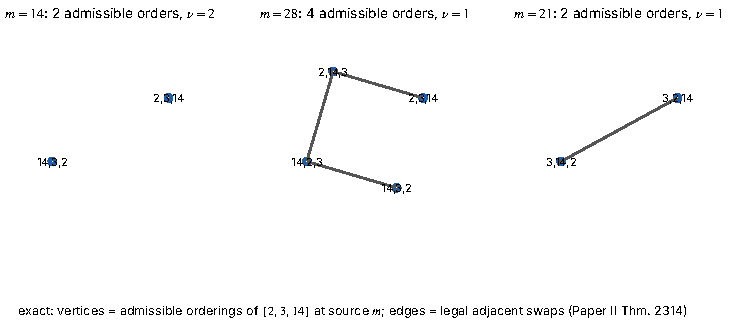
\includegraphics[width=\linewidth]{fig10_swap_components.pdf}
\caption{\textbf{Local swaps and globally disconnected history classes.} Swap graphs of the admissible orders of $\{2,3,14\}$ at the sources $14$, $28$, $21$ (\Src{II}{thm:2314}); the number of components is $\nu=2,1,1$. \emph{Exact; computed.}}\label{fig:swap}\end{figure}

\subsection{Cubes and homology}
A combinatorial cube of legal swaps is contractible once filled; the homology of the route complex of all histories to an integer records more. Paper~II proves that route complexes can have nontrivial higher-dimensional homology in suitable families (see \Src{II}{thm:sphere}, \Src{II}{thm:dual}); we use only the logical point that \emph{the presence of cubes does not decide the homology}, which is why the history side requires its own computations and cannot be read from $K(D(t))$ (\cref{prop:P5}).

\noindent\Cref{fig:loop} shows a history loop and a higher-dimensional void.

\begin{figure}[t]\centering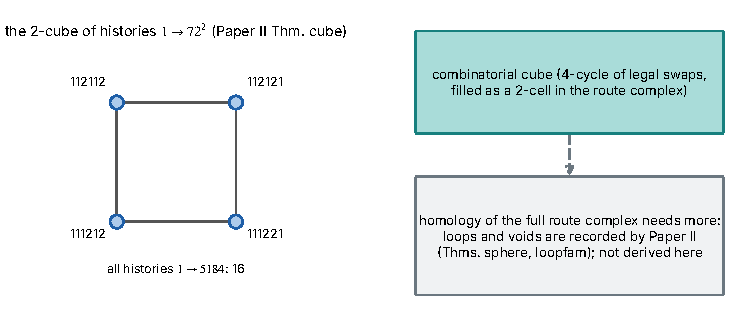
\includegraphics[width=\linewidth]{fig11_loop_void.pdf}
\caption{\textbf{A history loop and a higher-dimensional void.} Left: the 2-cube of histories $1\to5184$ (exact words). Right: what is and is not claimed; the homology of full route complexes is recorded in Paper~II. \emph{Left exact, right schematic.}}\label{fig:loop}\end{figure}
